  
\documentclass{beamer}
\usepackage{listings}
\lstset{
%language=C,
frame=single, 
breaklines=true,
columns=fullflexible
}
\usepackage{subcaption}
\usepackage{url}
\usepackage{tikz}
\usepackage{graphicx}
\usepackage{tkz-euclide} % loads  TikZ and tkz-base
%\usetkzobj{all}
\usetikzlibrary{calc,math}
\usepackage{float}
\newcommand\norm[1]{\left\lVert#1\right\rVert}
\renewcommand{\vec}[1]{\mathbf{#1}}
\newcommand{\R}{\mathbb{R}}
\newcommand{\C}{\mathbb{C}}
\providecommand{\brak}[1]{\ensuremath{\left(#1\right)}}
\providecommand{\abs}[1]{\vert#1\vert}
\providecommand{\fourier}{\overset{\mathcal{F}}{ \rightleftharpoons}}
\providecommand{\pr}[1]{\ensuremath{\Pr\left(#1\right)}}
\providecommand{\sbrak}[1]{\ensuremath{{}\left[#1\right]}}
\usepackage[export]{adjustbox}
\usepackage[utf8]{inputenc}
\usepackage{amsmath}
\usetheme{Boadilla}
\title{Research Paper Presentation}
\author{Kodavanti Rama Sravanth}
\institute{IITH}
\date{CS20BTECH11027}
\begin{document}
%
\begin{frame}
\titlepage
\end{frame}
\begin{frame}{Title and Authors}
%\frametitle{Prerequisites}
\begin{block}{Title}
On the Performance of Non-Orthogonal
Multiple Access in 5G Systems with
Randomly Deployed Users
\end{block}
\begin{block}{Authors}
\begin{itemize}
    \item Zhiguo Ding,Member,IEEE
    \item Zheng Yang,Senior Member,IEEE
    \item  Pingzhi Fan,Senior Member,IEEE
    \item  H. Vincent Poor,Fellow,IEEE
\end{itemize}
\end{block}
\end{frame}
\begin{frame}{}
\begin{block}{Abstract}
    \begin{itemize}
        \item The fourth generation of mobile networks,such as long term evolution are being deployed world wide and defining the next generation mobile network is receiving a lot of attention.
        \item Non Orthogonal Multiple Access has been recognized as a promising multiple access techniques for  fifth generation (5G)  networks.
        \item This paper describes the performance of NOMA over other access techniques in a downlink network with randomly deployed mobile users.
    \end{itemize}
    \end{block}
    \end{frame}
    \begin{frame}{}
    \begin{block}{Prerequisites}
       \begin{itemize}
           \item NOMA
           \item SIC
           \item Outage Probability
           \item Ergodic Rate
           \item Rayleigh Distribution
       \end{itemize}
    \end{block}
    \end{frame}
    \begin{frame}{Prerequisites}
    \begin{block}{Non Orthogonal Multiple Access(NOMA)}
    \begin{itemize}
        \item NOMA was proposed as a candidate radio access technology for 5G cellular systems.
        \item NOMA exploits superposition coding at the transmitter and successive interference cancellation (SIC) at the receiver to seperate the user data, thus multiplexing users in the power domain.
        \item NOMA has evolved as a spectral efficient,multiple access scheme so that it can cater to a large number of devices.
        \end{itemize}
    \end{block}
    \end{frame}
        \begin{frame}{Prerequisites}
      \begin{block}{Successive Interference Cancellation(SIC)}
            \begin{itemize} 
                 \item SIC is a technique used by receiver in wireless communication that allows decoding of two or more packets that arrived simultaneously.
        \item SIC is achieved by the receiver decoding the stronger signal first, subtracting it from the combined signal and then decoding the difference as the weaker signal.
        \item SIC enhances user security by using MAC address and IMEI ,Which are dedicated to a smartphone as a private keys
    \end{itemize}
    \end{block}
    \end{frame}
    \begin{frame}{Prerequisites}
    \begin{block}{Outage Probability(OP)}
       Outage Probability is defined as the probability that a given information rate is not supported i.e the probability that information rate is less than the required threshold information rate(where the value relates to the minimum signal to noise ratio (SNR) with in a cellular network), One can say that the receiver is out of range of Base Station (BS) in cellular communication.
    \end{block}
    \begin{block}{Ergodic Rate}
       Ergodic rate is defined as maximum achievable rate averaged over all the fading channels.
    \end{block}
\end{frame}
\begin{frame}{Prerequisites}
 \begin{block}{Rayleigh Distribution}
 \begin{itemize}
 \item Rayleigh distribution is a continuous probability distribution for non negative valued random variables. 
 \item The channels whose magnitude of the signal  through a transmission medium  varies according to Rayleigh distribution are called Rayleigh fading models.
 \item The probability density function of the Rayleigh distribution is :
 \begin{align}
     f(x;\sigma)=\frac{x}{\sigma^2}e^{-x^2/(2\sigma^2)}
 \end{align}
 \item The cumulative distribution function of the Rayleigh distribution is :
 \begin{align}
     F(x;\sigma)=1-e^{-x^2/2\sigma^2}
 \end{align}
 \end{itemize}
 \end{block}   
\end{frame}
\begin{frame}{Abbreviations}
\begin{center}
\begin{table}[h]
    \centering
    \scalebox{1}{
    \resizebox{\columnwidth}{!}{
\begin{tabular}{|c|c|}
\hline
\textbf{Abbreviation} &  \textbf{Meaning} \\
\hline
$h_{m}$ & Channel between $m$ th user and base station\\
\hline
$g_{m}$ & Rayleigh fading channel gain\\
\hline
$\alpha$ & Path loss factor \\
\hline
$d_{m}$ & Distance between user and base station\\
\hline
$s_{m}$ & Message for $m$ th user\\
\hline
$P$ & Transmission power\\
\hline
$a_{m}$ &Power allocation coefficient\\
\hline
$n_{m}$ & Additive noise for $m$ th user\\
\hline
$\rho$ & transmit SNR\\
\hline
$R_{m}$ & Achievable data rate for $m$ th user \\
\hline
$\Bar{R_{m}}$ & Targeted data rate for $m$ th user\\
\hline
$R_{j\rightarrow m}$ & Data rate of $m$ th user to detect the $j$ th user message.\\
\hline
\end{tabular}
}
}
    \caption{Abbreviations used  in the experiment}
    \label{Abbreviation table}
\end{table}
\end{center}
\end{frame}
\begin{frame}{Formulae}
   \begin{center}
\begin{table}[h]
    \centering
    \scalebox{1}{
    \resizebox{10cm}{!}{
\begin{tabular}{|c|c|}
\hline
\textbf{Abbreviation} &  \textbf{Formula} \\
\hline
$\phi_j$ & $2^{\bar{R_j}}-1$\\
\hline
$\psi_j$ & $\frac{\phi_j}{\rho(a_j-\phi_j\sum_{i=j+1}^{M}a_i)}$ for $j<M$\\
\hline
$\psi_M$ & $\frac{\phi_M}{\rho a_M}$\\
\hline
$\psi_m ^{*}$ & $\max_{}\psi_1,....\psi_m$\\
\hline
$E_{M,M}^c$ & $\rho \abs{h_m}^2 a_M >\psi_M$\\
\hline
\end{tabular}
}
}
    \caption{Formulae used  in the experiment}
    \label{Formula table}
\end{table}
\end{center} 
\end{frame}
\begin{frame}{}
\begin{block}{NOMA Transmission Protocol}
\begin{itemize}
  \item Let us consider a cellular downlink in which base station is at the centre of disk '$D$' with radius $R_{D}$ and '$M$' users are uniformly distributed within the disk. Then the channel $h_{m}$ is given by 
   \begin{align}
       h_{m}=\frac{g_{m}}{\sqrt{1+d_{m}^\alpha}}
   \end{align}
   \item The channels are sorted as:
   \begin{align}
       \abs{h_1}^2\leq \abs{h_2}^2 ......\leq\abs{h_M}^2
   \end{align}
   \item The power allocation coefficients are sorted as:
   \begin{align}
       a_1\geq a_2....\geq a_M
   \end{align}
   \end{itemize}
   \end{block}
   \end{frame}
   \begin{frame}
     \begin{block}{NOMA Transmission Protocol}
   \begin{itemize}
  \item  According to NOMA protocol, Observation for the $m$ th user is given by
   \begin{align}
       y_{m}=h_{m}\sum_{i=1}^{M}\sqrt{a_{i}P}s_{i}+n_{m}
   \end{align}
   \item As  Successive Interference Cancellation (SIC) is carried out at all the users, m th user will detect $i$ th user message for $i<m$ and for $i>m$ it will be treated as a noise.
   \item So,The data rate achievable for mth user, 1$\leq m\leq  M-1 $  is given by:
     \begin{align}
       R_{m}=\log\brak{1+\frac{\rho\abs{h_{m}}^{2} a_{m}}{\rho\abs{h_{m}}^2\sum_{i=m+1}^{M}a_{i}+1}}\label{eq:7}
   \end{align}
  \end{itemize}
  \end{block}
\end{frame}
\begin{frame}
\begin{block}{NOMA Transmission Protocol}
\begin{itemize}

 \item Also, The data rate of $m$ th user to detect the $j$ th   ($j\leq m$) user message is:
 \begin{align}
     R_{j\rightarrow m}=\log\brak{1+\frac{\rho\abs{h_{m}}^{2} a_{j}}{\rho\abs{h_{m}}^2\sum_{i=j+1}^{M}a_{i}+1}}\label{eq:8}
 \end{align}
 \item The two equations \eqref{eq:7} and \eqref{eq:8} are obtained if  and only if the condition $R_{j\rightarrow m} \geq \bar{R_j}$ is true.
   \item Rate of $M$ th user is given by:
   \begin{align}
       R_M=log(1+\rho \abs{h_M}^2 a_M)
   \end{align}
   \item Consequently sum rate achieved by NOMA is \begin{align}
       R_{sum}=\sum_{m=1}^{M-1} \log\brak{1+\frac{\rho\abs{h_{m}}^{2} a_{m}}{\rho\abs{h_{m}}^2 \Bar{a_m}+1}}+ log(1+\rho \abs{h_M}^2 a_M)
   \end{align} 
   \end{itemize}
\end{block}
\end{frame}
    \begin{frame}{}
\begin{block}{Density Functions of Channel gains}
\begin{itemize}
  \item The channel gain $h$ contributes its part in evaluation of outage probability and ergodic sum rate.
  \item As the users are uniformly distributed over the disk and small scale fading is Rayleigh distributed,The CDF of the channel gain $\abs{h}^2$ is given by:
  \begin{align}
      F_{h^2} (y)= \frac{2}{R_{D}^2} \int_{0}^{R_D} \brak{1-e^{-(1+z^\alpha)y}} z dz 
  \end{align}
  \item By Gaussian-Chebyshev quadrature we can approximate the integral as 
  \begin{align}
      F_{h^2} (y) \approx \frac{1}{R_D} \sum_{n=1}^{N} \omega_{n} \times  g(\theta_{n})
  \end{align}
  \end{itemize}
  \end{block}
  \end{frame}
  \begin{frame}{}
  \begin{block}{Density Functions of Channel gains}
  \begin{itemize}
  \item The PDF of the channel gain can be approximated as 
  \begin{align}
      f_{h^2} (y) \approx \frac{1}{R_D} \sum_{n=1}^{N} \beta_{n} e^{-c_n y}
  \end{align}
  Where,
  \item $g(x)=\sqrt{1-x^2}(1-e^{-c_n y})(\frac{R_D}{2} x+\frac{R_D}{2})$
  \item $c_n=1+\brak{\frac{R_D}{2}\theta_n+\frac{R_D}{2}}^\alpha$
  \item $\omega _n=\frac{\pi}{N}$
  \item $\theta_n=cos(\frac{2n-1}{2N}\pi)$
  \item $\beta_n=\omega_n\sqrt{1-\theta_n^2}\times(\frac{R_D}{2}\theta_n+\frac{R_D}{2})c_n$
  \end{itemize}
   \end{block}
    \end{frame}
    \begin{frame}
        \begin{block}{Outage Performance of NOMA}
        \begin{itemize}
            \item The outage events of $m$ th user is defined as the event that $m$ th user cannot detect the $j$ th user's message.So the event $E_{m,j}$ is
            \begin{align}
            E_{m,j}\cong \brak{R_{j\rightarrow m}< \bar{R_j}}
            \end{align}
            \item The outage probability of $m$ th user can be expressed as :
            \begin{align}
                P_{m}^{out}=1-P({E_{m,1}^c} \cap ........\cap {E_{m,m}^c })
            \end{align}
            \item The events $E_{m,j}^c$ can be expressed as :
            \begin{align}
                E_{m,j}^c &=\Bigg\{\frac{\rho\abs{h_{m}}^{2} a_{j}}{\rho\abs{h_{m}}^2\sum_{i=j+1}^{M}a_{i}+1}> \phi_j\Bigg\}\\
                &=\Bigg\{\rho\abs{h_m}^2 \brak{a_j-\phi_j\sum_{i=j+1}^{M}a_i}>\phi_j\Bigg\}\label{eq:17}
            \end{align}
        \end{itemize}
        \end{block}
        \end{frame}
        \begin{frame}{}
            \begin{block}{Outage Performance of NOMA}
            \begin{itemize}
                \item The  equation \eqref{eq:17} is derived if and only if the  below condition is true \begin{align}
                a_j >\phi_j\sum_{i=j+1}^{M} a_i \label{eq:18}
                \end{align}
                \item When $\rho \rightarrow \infty$ ,$\psi_m^{*}\rightarrow 0$ the outage probability is given as i.e high SNR approximation of OP is :
                \begin{align}
                    P_m^{out} \rightarrow \frac{1}{\rho^m} \label{eq:19}
                \end{align}
                \item From \eqref{eq:19}  we can say that  $m$ th user will experience a diversity order of '$m$'.This is better than conventional orthogonal MA scheme whose diversity order is one. 
                \item So, NOMA will achieve better spectral efficiency and user fairness as all the users are served at same time,frequency.
            \end{itemize}
            \end{block}
        \end{frame}
        \begin{frame}{Outage Performance of NOMA}
            \begin{block}{Drawback}
            \begin{itemize}
                \item The superior outage performance of NOMA is worthy pointing out,But it is conditioned  to the constraint of \eqref{eq:18}.
                \item When such a condition is not satisfied ,e.g $a_j \leq \phi_j\sum_{i=j+1}^{M} a_i$ \\ then the user's outage probability is always one,  \\i.e $P_m^{out}=1$
                \item  We can consider this as a drawback of NOMA.
            \end{itemize}
            \end{block}
        \end{frame}
        
        \begin{frame}{Graphs of Outage Performance vs SNR}
       
            \begin{figure}[ht]
    \centering
    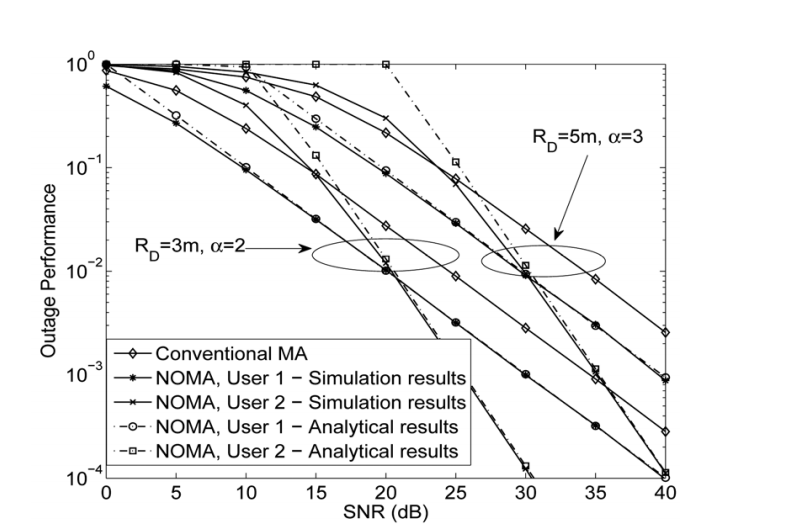
\includegraphics[width=0.7\textwidth]{Fig-1.png}
    \caption{OP of MA techniques with $\bar{R_1}=0.1$ BPCU,$\bar{R_2}=0.5$ BPCU}
    \label{OP vs SNR 1}
\end{figure}
        \end{frame}
               \begin{frame}{Graphs of Outage Performance vs SNR}
       
            \begin{figure}[ht]
    \centering
    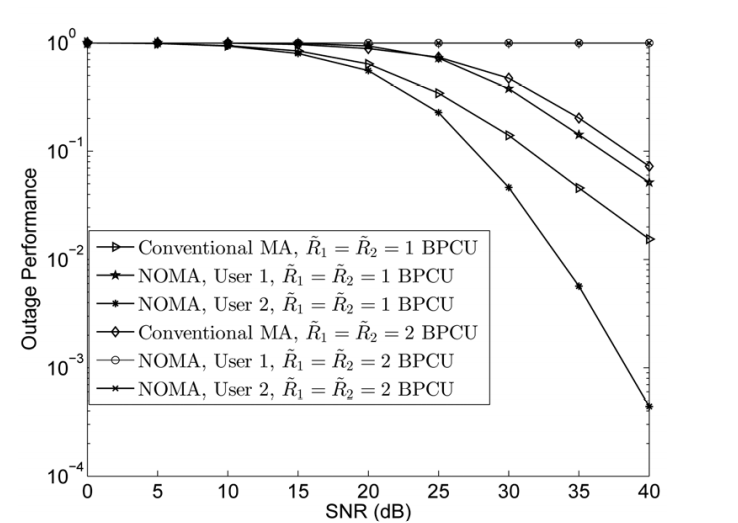
\includegraphics[width=0.7\textwidth]{Fig-2.png}
    \caption{OP of MA techniques with $R_D=5$ m ,$\alpha=3$ }
    \label{OP vs SNR 2}
\end{figure}
        \end{frame}
        \begin{frame}{}
            \begin{block}{Ergodic Sum Rate of NOMA}
            \begin{itemize}
                \item The ergodic sum rate when $R_j=\bar{R_j}$ is given by
                
                    \begin{equation}
                   \begin{split} R_{avg}=\sum_{m=1}^{M} \int_{0} ^{\infty} log\brak{1+\frac{x \rho a_m}{x\rho \bar{a_m}+1}} f_{\abs{h_m}^2} (x) dx\\
                    +\int_{0} ^{\infty} log(1+\rho x a_M) f_{\abs{h_M}^2} (x) dx
                    \end{split}
                    \end{equation}
        \item The exact expression of above integral is difficult to obtain.So we do approximation with $M \rightarrow \infty$
        \begin{align}
            R_{avg} \rightarrow log(\rho log(log(  M)))
        \end{align}
        \item NOMA will achieve the same asymptotic performance as the opportunistic scheme,but NOMA can offer better fairness since all the users are served simultaneously.
            \end{itemize}
            \end{block}
        \end{frame}
               \begin{frame}{Graphs of Ergodic Sum Rate vs SNR}
       
            \begin{figure}[ht]
    \centering
    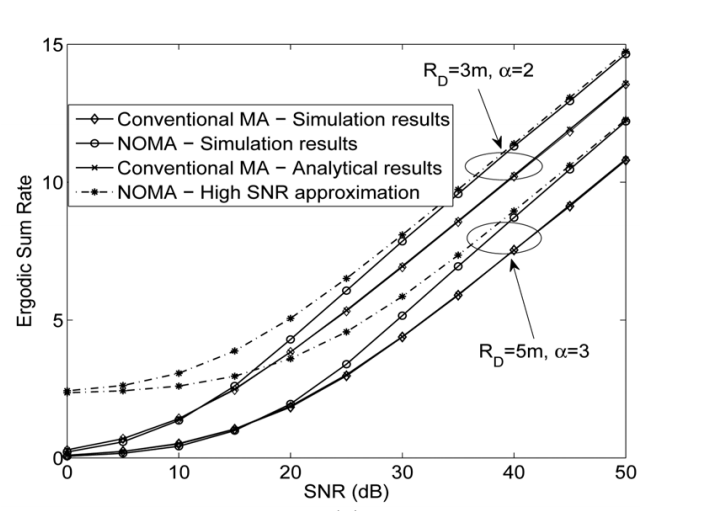
\includegraphics[width=0.7\textwidth]{Fig-3.png}
    \caption{Ergodic Sum Rate achieved by MA techniques with M=2}
    \label{Ergodic vs SNR 1}
\end{figure}
        \end{frame}        \begin{frame}{Graphs of Ergodic Sum Rate vs SNR}
       
            \begin{figure}[ht]
    \centering
    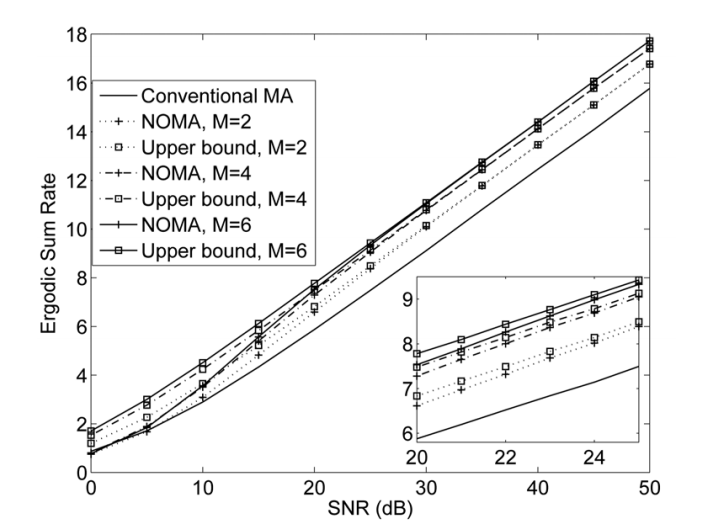
\includegraphics[width=0.7\textwidth]{Fig-4.png}
    \caption{Ergodic Sum Rate achieved by MA techniques with R=5 m and $\alpha=2$}
    \label{Ergodic vs SNR 2}
\end{figure}
        \end{frame}
        \begin{frame}
            \begin{block}{Conclusions}
            \begin{itemize}
                \item In this paper we have demonstrated that NOMA can achieve better outage performance than the orthogonal MA
                  techniques, under the condition that the users rates and power
          coefficients are carefully chosen.
          \item Also,NOMA can achieve a superior ergodic sum rate, and is asymptotically equivalent to the opportunistic MA technique
            \end{itemize}
            \end{block}
            \begin{block}{Potential Drawbacks}
            \begin{itemize}
                \item NOMA introduces additional complexity due to the use of SIC.
                \item The performance gain of NOMA at low SNR is insignificant.
            \end{itemize}
            \end{block}
        \end{frame}
        \begin{frame}
   \centering
    \textcolor{violet}{\Huge{\textbf{THANK YOU}}}
 \begin{figure}
 \centering{
    
\includegraphics[width=0.4\textwidth]{logo.png}}
    \label{logo}
\end{figure}
\end{frame}
\end{document}